\begin{figure}[htbp]
\centering
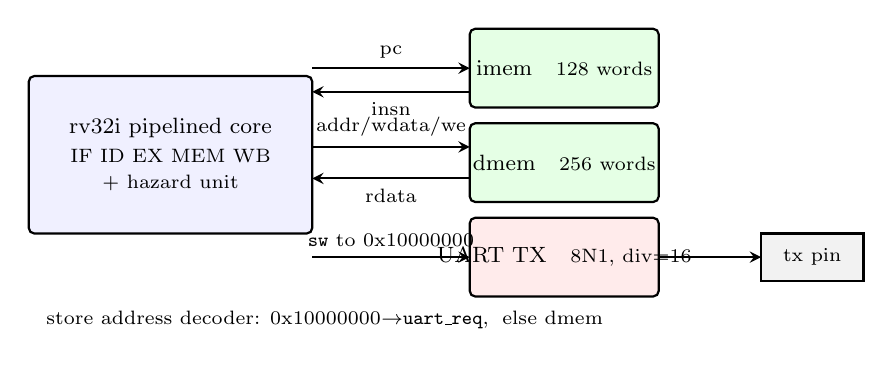
\begin{tikzpicture}[font=\footnotesize, >=stealth, x=1cm, y=1cm]
  \draw[thick, fill=blue!6, rounded corners=2pt] (0,1.4) rectangle (3.6,3.4);
  \node[align=center] at (1.8,2.4) {rv32i pipelined core\\[1pt]
    \scriptsize IF ID EX MEM WB\\ \scriptsize + hazard unit};
  \draw[thick, fill=green!10, rounded corners=2pt] (5.6,3.0) rectangle (8.0,4.0);
  \node at (6.8,3.5) {imem\quad\scriptsize 128 words};
  \draw[thick, fill=green!10, rounded corners=2pt] (5.6,1.8) rectangle (8.0,2.8);
  \node at (6.8,2.3) {dmem\quad\scriptsize 256 words};
  \draw[thick, fill=red!8, rounded corners=2pt] (5.6,0.6) rectangle (8.0,1.6);
  \node at (6.8,1.1) {UART TX\quad\scriptsize 8N1, div=16};
  \draw[thick, fill=gray!10] (9.3,0.8) rectangle (10.6,1.4);
  \node at (9.95,1.1) {\scriptsize tx pin};
  \draw[->, thick] (3.6,3.5) -- node[above]{\scriptsize pc} (5.6,3.5);
  \draw[->, thick] (5.6,3.2) -- node[below]{\scriptsize insn} (3.6,3.2);
  \draw[->, thick] (3.6,2.5) -- node[above]{\scriptsize addr/wdata/we} (5.6,2.5);
  \draw[->, thick] (5.6,2.1) -- node[below]{\scriptsize rdata} (3.6,2.1);
  \draw[->, thick] (3.6,1.1) -- node[above]{\scriptsize \texttt{sw} to 0x10000000} (5.6,1.1);
  \draw[->, thick] (8.0,1.1) -- (9.3,1.1);
  \node[align=left, anchor=west, font=\scriptsize] at (0.1,0.3)
    {store address decoder: 0x10000000$\to$\texttt{uart\_req},\; else dmem};
\end{tikzpicture}
\caption{The ch08 SoC: the pipelined core, instruction memory, data
memory, and a memory-mapped UART. One extra address-compare line
turns an ordinary \texttt{sw} into a serial transmission.}
\label{fig:soc08}
\end{figure}
